\section{Tails Analysis}

At this point we should have notice that the real danger of investments does not resides solely within the standard concept of dispersion (standard deviation), nor within the ratio between return and dispersion. The true risk dwells in the worst case scenarios of the distributions, the tails. Where accumulated or great losses may strike down the whole investment plan. Hence, in order to address the risk analysis of any savings strategy, we need to take a closer look at the tails of their distributions. 


Taking a close look at Figure \ref{fig:both_fw}, we are not able to clearly state which one is \textit{less risky}. So far, we have been comparing the values of Expected Shortfall in order to get a sense of the risk. But, since the ES is actually just the average of the tail of the distribution, we will now discuss how we can pursue a more in-depth analysis for the distribution of those tails.

In this section, we will go one step further and try to fit some specific distribution to those tails. This way we will be able to see in more detail the behaviour of the losses of our strategies, and set more accurate risk measures.

\subsection{Definition of \textit{Tail}}

First things first. What is \emph{the} Tail of a distribution? The tail of a distribution is not a precisely defined term; it can have many different forms and definitions. Generally, the \textit{tail} is considered a broad term to name the extreme parts of a distribution. In other words, there is not some specific place where you stop being in the middle of the distribution and start being in the tail, and where to put that line is up to every case.

Let's say that we plot a distribution $Y$, the loss of a savings plan (note that negative losses imply profits). We decide to put the distinction between middle and tail at some point named $u$, so the tail would be everything that lands within $Y>u$.

If we understand the tail of a distribution as a distribution itself, we can move that tail to the origin and normalise its area. Thus, being positively defined as

\begin{align}
    Z = \qty(Y-u | Y>u)
\end{align}.

Once we have this definition, we can easily define the probability density as

\begin{align}
    F_Z(z)  &=  P(Z < z) = P\qty(Y-u < z | Y>u)  \\
            &=  P\qty(Y<z+u | Y>u) \\
            &= \frac{P\qty(Y<z+u, Y>u)}{P\qty(Y>u)}
\end{align}

And thus, deriving this expression we find that, for every $z>0$,

\begin{align}
    f_z(z) = \frac{f_y\qty(z+u)}{1-F_y(u)}\textit{.}
\end{align}

Interesting thing about this result, is that we can analytically relate the distribution of the tail $f_z(z)$ with the whole original distribution $f_y(z)$.

Therefore, we can say that, if the distribution of the losses obtained is $Y$, our tail could be defined as

\begin{align}
    F_u(y) = \qty( Y - u \leq y| Y > u ) \emph{.}
\end{align}

The Pickands-Balkema-de Haan theorem states that for a large class of distributions $X$, exists $u$ such as that $F_u$ is well approximated by the Generalized Pareto Distribution (GPD) $G$. Where the standard cumulative distribution function of the GPD can be defined as:


\[F_{\xi}(y) = \left\{
  \begin{array}{lr}
    1 - \qty(1 + \xi y)^{\sfrac{-1}{\xi}} & : \xi \neq 0\\
    1 - e^{-y} & : \xi = 0
  \end{array}
\right. \emph{.}
\]

Thus, we can seek that point $u$ from which our tail could fit a GPD. That would imply that, from that point $u$ forward, the distribution follows a GPD. The kind of GPD would be determined by the value of $\xi$. This number, usually called \emph{Extreme Value Index}, that determines  the shape of the distribution. The larger the value of $\xi$, the thicker the tail grows, and the slowly it converges to zero. In general:

\begin{itemize}
    \item $\xi > 0$. The tail does not converge to zero, ever. Power-law
    \item $\xi = 0$. The tail converges to zero at infinity. Exponential
    \item $\xi < 0$. The tail converges to zero in a finite point.
\end{itemize}

In what risk analysis concerns, the value of $\xi$ is crucial. Since we are studying the risk of a strategy looking at the tail of distributions where distribution are the frequency of losses, we could think that the wider or thicker the tail, the riskier the strategy. 

\subsection{Extreme Value Analysis: Fitting a General Pareto Distribution}

Let us repeat the simulation for the CPPI, using $\pi = 0.1$, and plot the histogram of its losses as an example.

\begin{figure}[H]
    \centering
    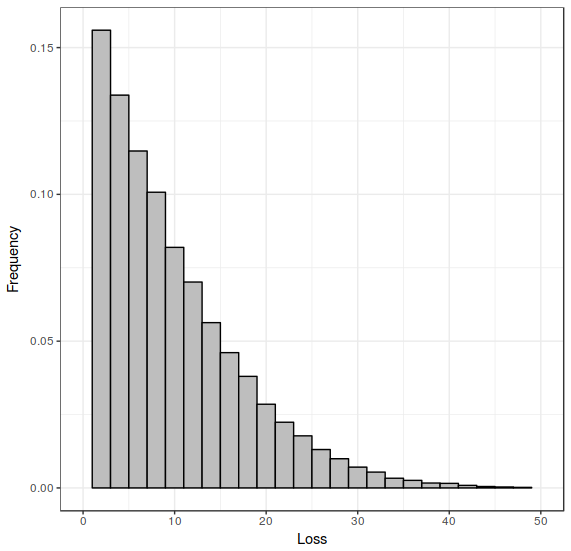
\includegraphics[scale=0.75]{images/cppi-losses-hist.png}
    \caption{Frequency Histogram of the losses of the CPPI strategy. Using $\pi = 0.1$, $\alpha = 0.0343$, $\sigma = 0.1544$ and $1000000$ simulations.}
    \label{fig:cppi-losses-histogram}
\end{figure}

If we now plot that density as points in a logarithmic scale, we might see something like the following:

\begin{figure}[H]
    \centering
    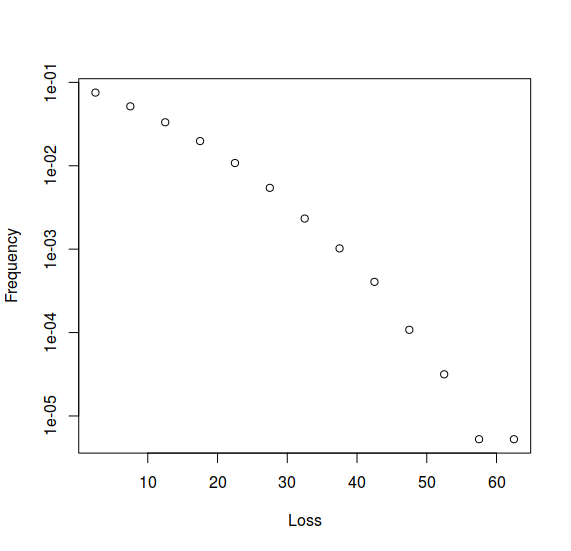
\includegraphics[scale=0.75]{images/cppi-dens-points.png}
    \caption{Density Distribution of the losses of the CPPI strategy in a logarithmic scale. Using $\pi = 0.1$, $\alpha = 0.0343$, $\sigma = 0.1544$ and $1000000$ simulations.}
    \label{fig:cppi-dens-points}
\end{figure}

Now, we could try to add here the Complementary Cumulative Distribution Function of a Generalized Pareto Distribution, and see if it fits to our distribution as it is now.

\begin{figure}[H]
    \centering
    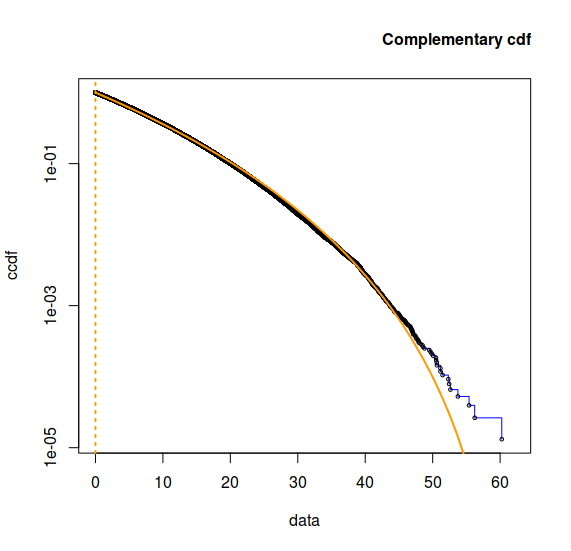
\includegraphics[scale=0.75]{images/cppi-ccdf-0.png}
    \caption{Density Distribution of the losses of the CPPI strategy in a logarithmic scale. Using $\pi = 0.1$, $\alpha = 0.0343$, $\sigma = 0.1544$ and $1000000$ simulations.}
    \label{fig:cppi-ccdf-0}
\end{figure}

Clearly, we can see how badly it fits for larger numbers. This indicates that our distribution is not following a GPD. Nevertheless, we can still find a proper $u$ for which it would.




\subsection{Convergence of the Expected Shortfall}

So far, we have addressed the necessity of studying the tail of loss danger using the Expected Shortfall. It is quite straightforward and it easily assesses the risk of the tail. But since it is nothing more than a simple mean, it can arise some issues. 

We talked about how the tail of a distribution can be considered a distribution by itself. Thus, the mean of the tail intends to be a summary statistic of this distribution. Despite that, we know that the arithmetic mean is not always a good summary statistic for every given distribution. There are some distributions from which the mean is not the best suited statistic to get a reliable feel of its \emph{general tendency}, especially on very skewed distributions.

Moreover, without previous knowledge about the distribution we may encounter, it exists the possibility of facing a distribution whose arithmetic mean does not exist. This possibility arises a very disturbing problem: The computed value of the Expected Shortfall should not exist. Since we are working with simulated data, and thus finite numbers, we will never face an infinite arithmetic mean. This implies that in order to ensure the reliability of the Expected Shortfall, we first need to check whether its computation makes sense or not.

In Figure \ref{fig:loss_both} we see the density curve of the loss tails of both methods. If we compute the histogram and set the bars of the histogram as points, we can build a scatterplot. 
In Figure \ref{fig:lm-tails} we can see this scatter plot of their logarithmic density points. It is of great interest noticing that, whereas both tails follow a linear model quite accurately (after taking logarithms), the \textit{Alternative} scheme has a much sharper descending trend. Which would mean that its \textit{Expected Shortfall} is far less likely to be infinite in any analytical distribution. This suggests us that the computed value of the Expected Shortfall is much more reliable for the \textit{Alternative} scheme than for the CPPI one.

\begin{figure}[h]
    \centering
    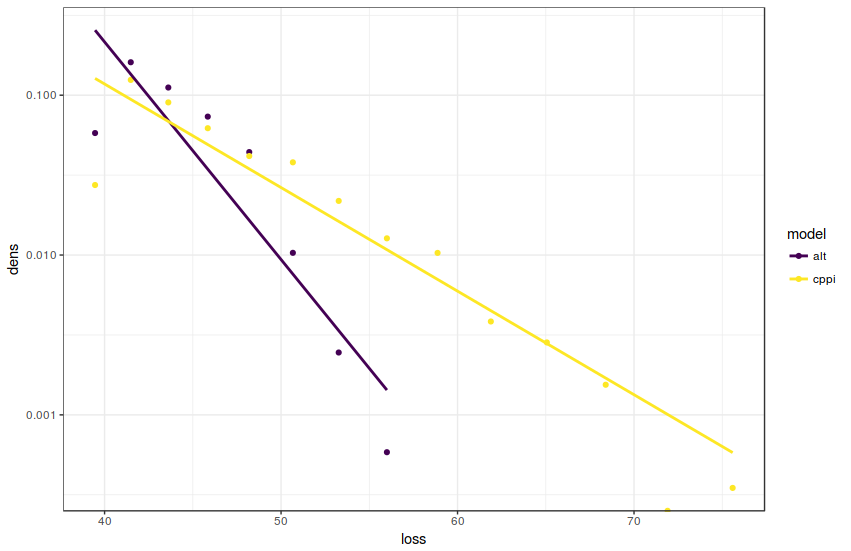
\includegraphics[scale=0.5]{images/lm_tails.png}
    \caption{Scatter plot and linear regression of the logarithm of the density points of the \textit{CPPI} and \textit{Alternative} methods.}
    \label{fig:lm-tails}
\end{figure}

